ld\chapter{Result}
\section{Experimentations}
The experimentation based on a machine equipped with Intel(R) Core(TM) i7-4790 CPU 3.6GHz, 16 GB of RAM. For each dataset, it includes 293 images(3264 x 2448). 
\subsection{The bad files}
In some cases, program can not estimate the landmarks because the scene image is empty or the segmentation from scene image is bad. The bad images showed as below:
\begin{multicols}{2}
\begin{itemize}
\item Md 091.JPG
\item Md 140.JPG
\item Md 146.JPG (empty image)
\item Md 169.JPG
\item Md 238.JPG (empty image)
\item Md 283.JPG
\item Mg 003.JPG (empty image)
\item Mg 105.JPG
\item Mg 110.JPG
\item Mg 112.JPG
\item Mg 146.JPG
\item Mg 153.JPG
\item Mg 168.JPG
\item Mg 170.JPG
\item Mg 211.JPG
\item Mg 222.JPG
\item Mg 248.JPG (empty image)
\end{itemize} 
\end{multicols}
\subsection{Parameters}
In the program, we have used the parameters for the methods:
\begin{itemize}
\item The ratio between \textit{lower threshold} and \text{upper threshold} used in Canny algorithm to obtain the edge is 1:3 (in class \textit{Image}, method \textit{getEdges}). The lower value is 1 * \textit{threshold} value and the upper value is 3 * \textit{threshold} value. The \textit{threshold} value has been identified by analysing the histogram of image. The range of lower value and upper value can be from 0 to 255, however, we need to indicate a reasonable value to get the best segmentation.
\item The angle and distance accuracy used in constructing the PGH matrix and calculate the measure distance between PGHs. The angle accuracy can be 90 (0.5 * 180), 180, 360 (2 * 180), 720(4 * 180), 1080(6 * 180), 2160(12 * 180) degree. The distance accuracy can be 250, 500 or 1000 columns. The default value in program is 180 degree for angle accuracy, and 250 for the distance accuracy. 
\item During apply the probabilistic hough transform, to save processing time during training, we just consider the pair of closet lines. And the parameters used to indicate the closet line are (used in method \textit{closetLine}, class \textit{PHoughTransform} ):
	\begin{itemize}
		\item Length of each line greater than \textbf{60} pixels
		\item Angle between two lines greater than \textbf{15} degree
		\item Perpendicular distance from one of two endpoints of a line to other line less than \textbf{5} pixel.
	\end{itemize}
And the condition to predicate two pair of lines are similar (used in method \textit{similarPairLines}, class \textit{PHoughTransform}):
	\begin{itemize}
		\item Subtraction between angle of two pair of lines is less than \textbf{1}
		\item Subtraction between ratio couple of scene lines and reference lines is less than \textbf{1}
		\item Subtraction between distance of two pair of lines is less than \textbf{2}
	\end{itemize}
\item The size of bounding box around reference landmarks used for estimating landmarks by cross-correlation method or compute the estimated centroid is \textit{400} pixels (used in method \textit{crossCorrelation and crossCorrelationDistance}, class \textit{ImageViewer})
\item The size of bounding box around reference landmarks and estimated landmarks used for refine the estimated landmarks or compute the estimated centroid are \textit{400} pixels and \textbf{1400} pixels, respective.(used in method \textit{getLandmarks and tplMatchingDistance}, class \textit{ImageViewer})
\end{itemize}
\section{Results}
The landmarks estimated automatically based on two method: \textit{cross-corrlelation} (called method 1) and \textit{the proposed method} (called method 2). And the result obtained from the method 2 is better than the result from the method 1.
\begin{figure}[h!]
\centering
\subfloat[The scene image]{\label{fig:pht_1}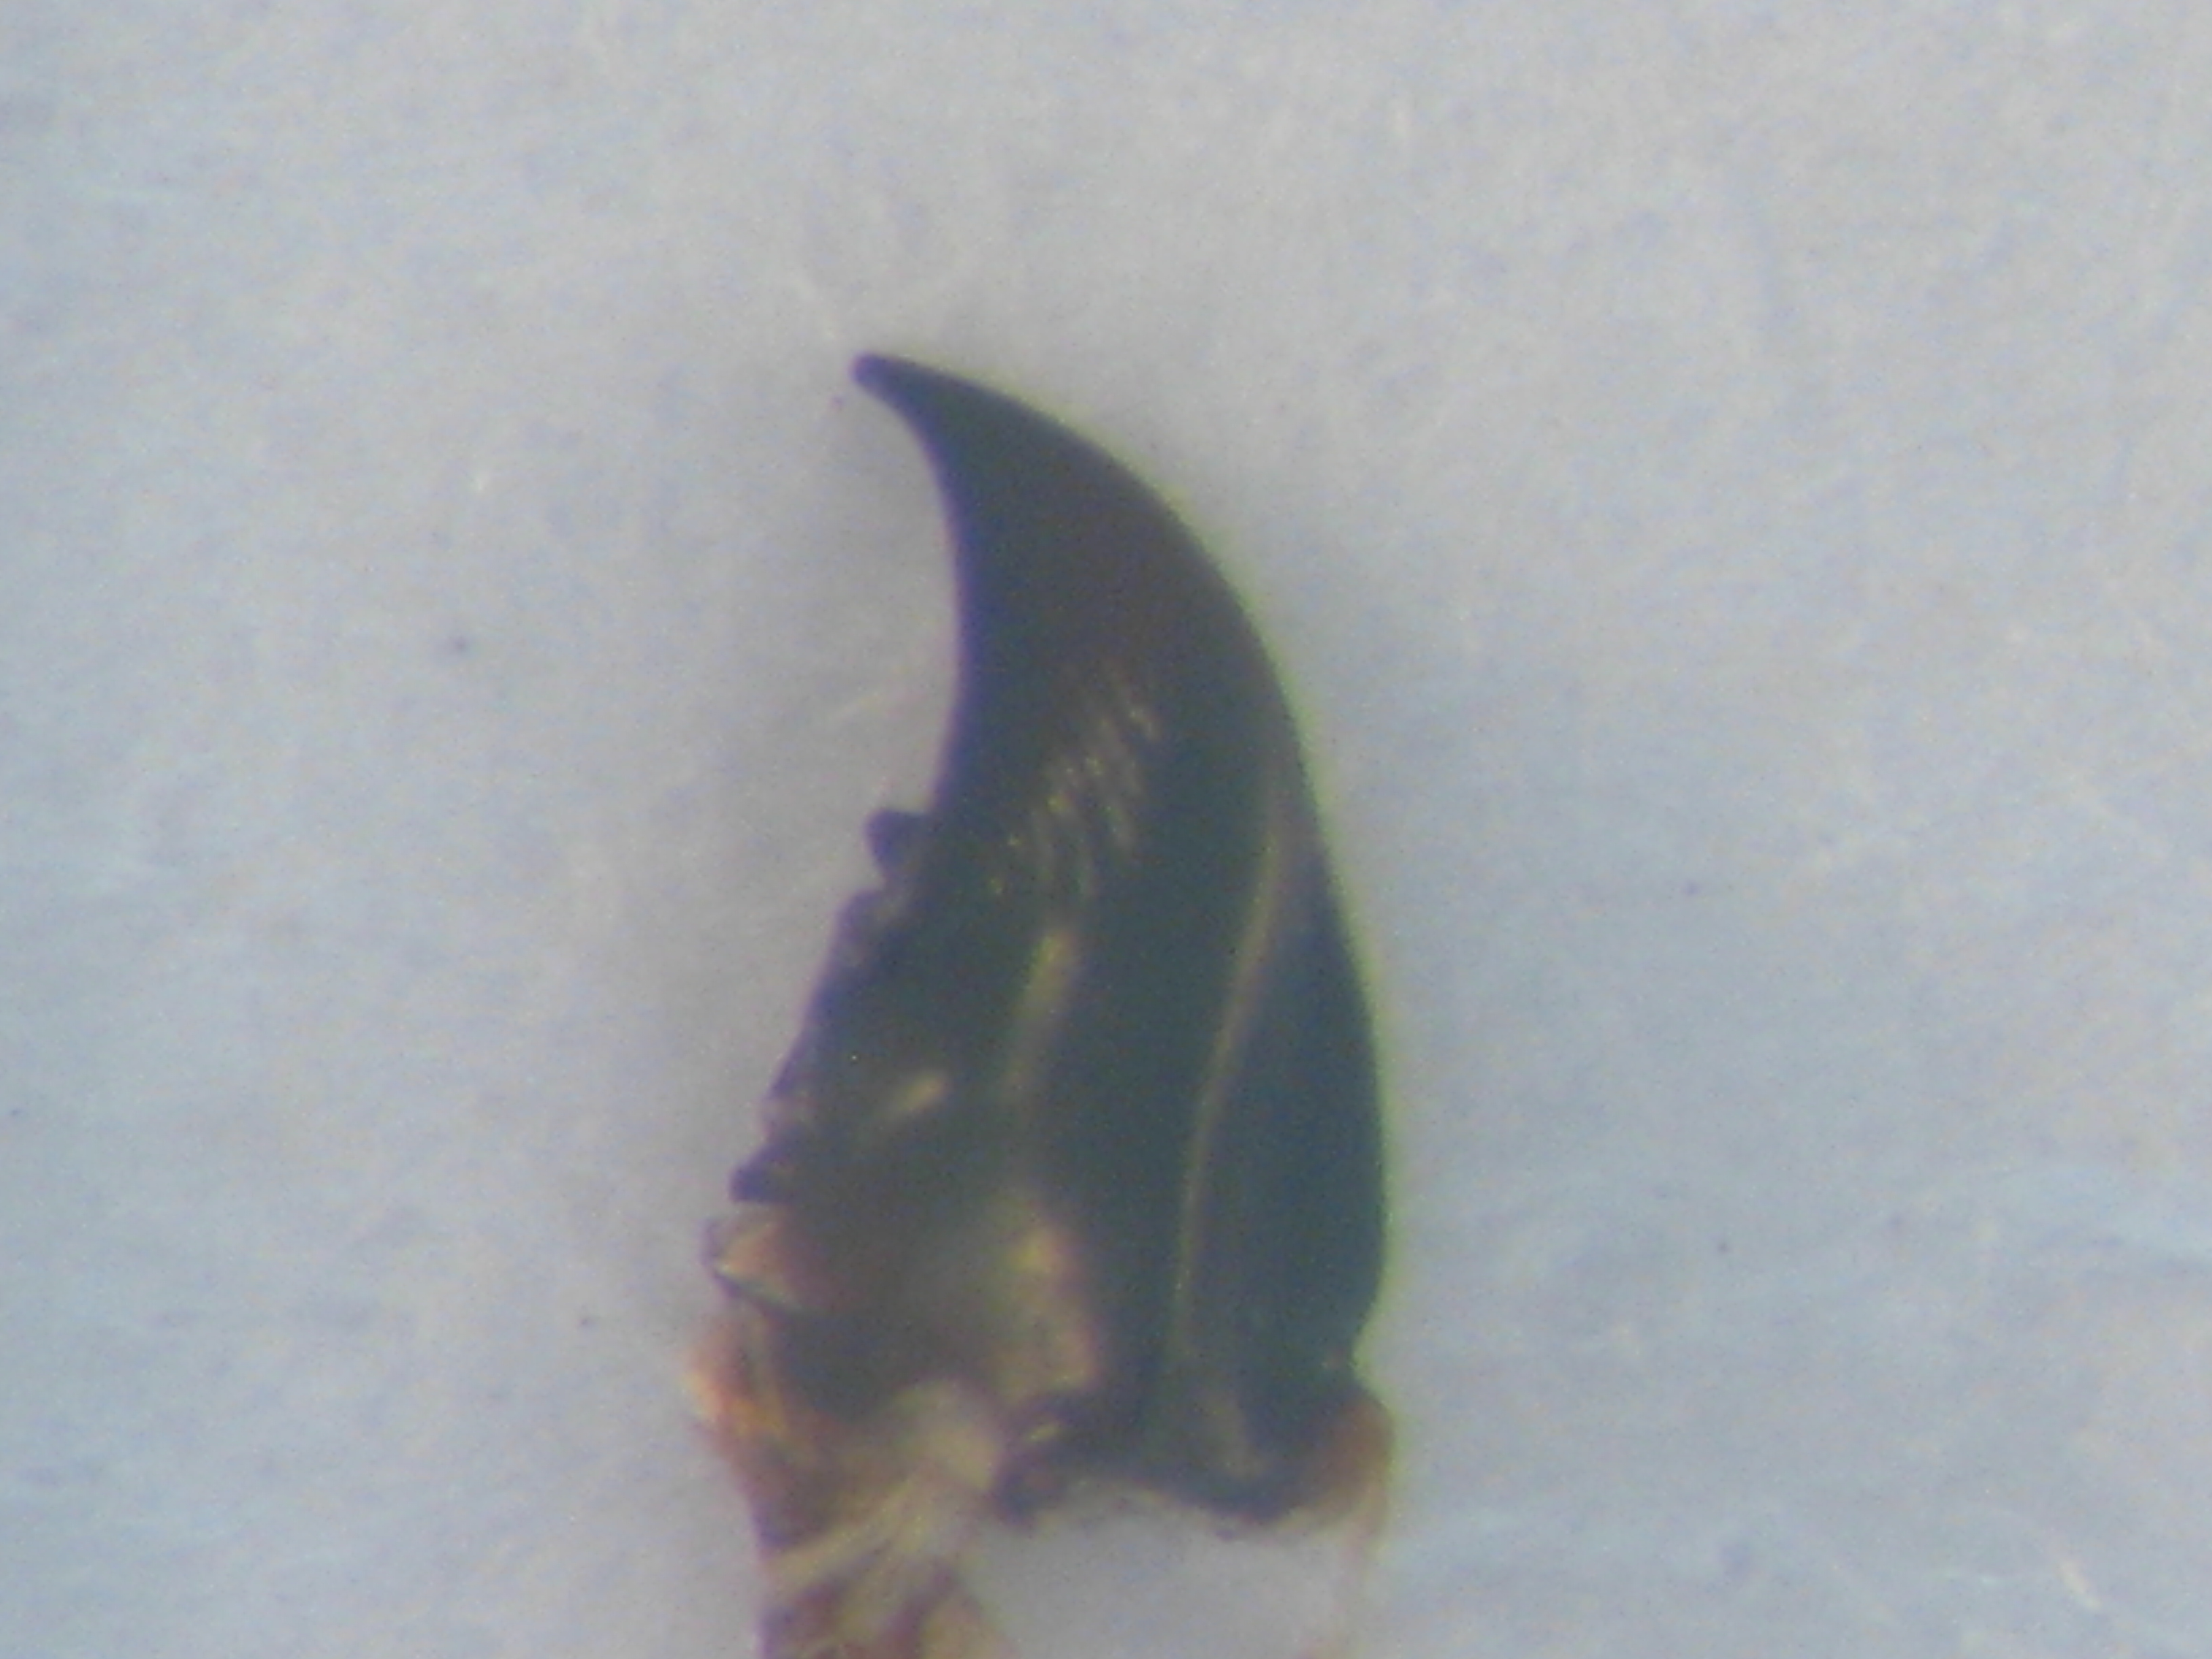
\includegraphics[width=0.45\textwidth]{./images/md32}}~~
\subfloat[The scene image with estimated landmarks ]{\label{fig:pht_2}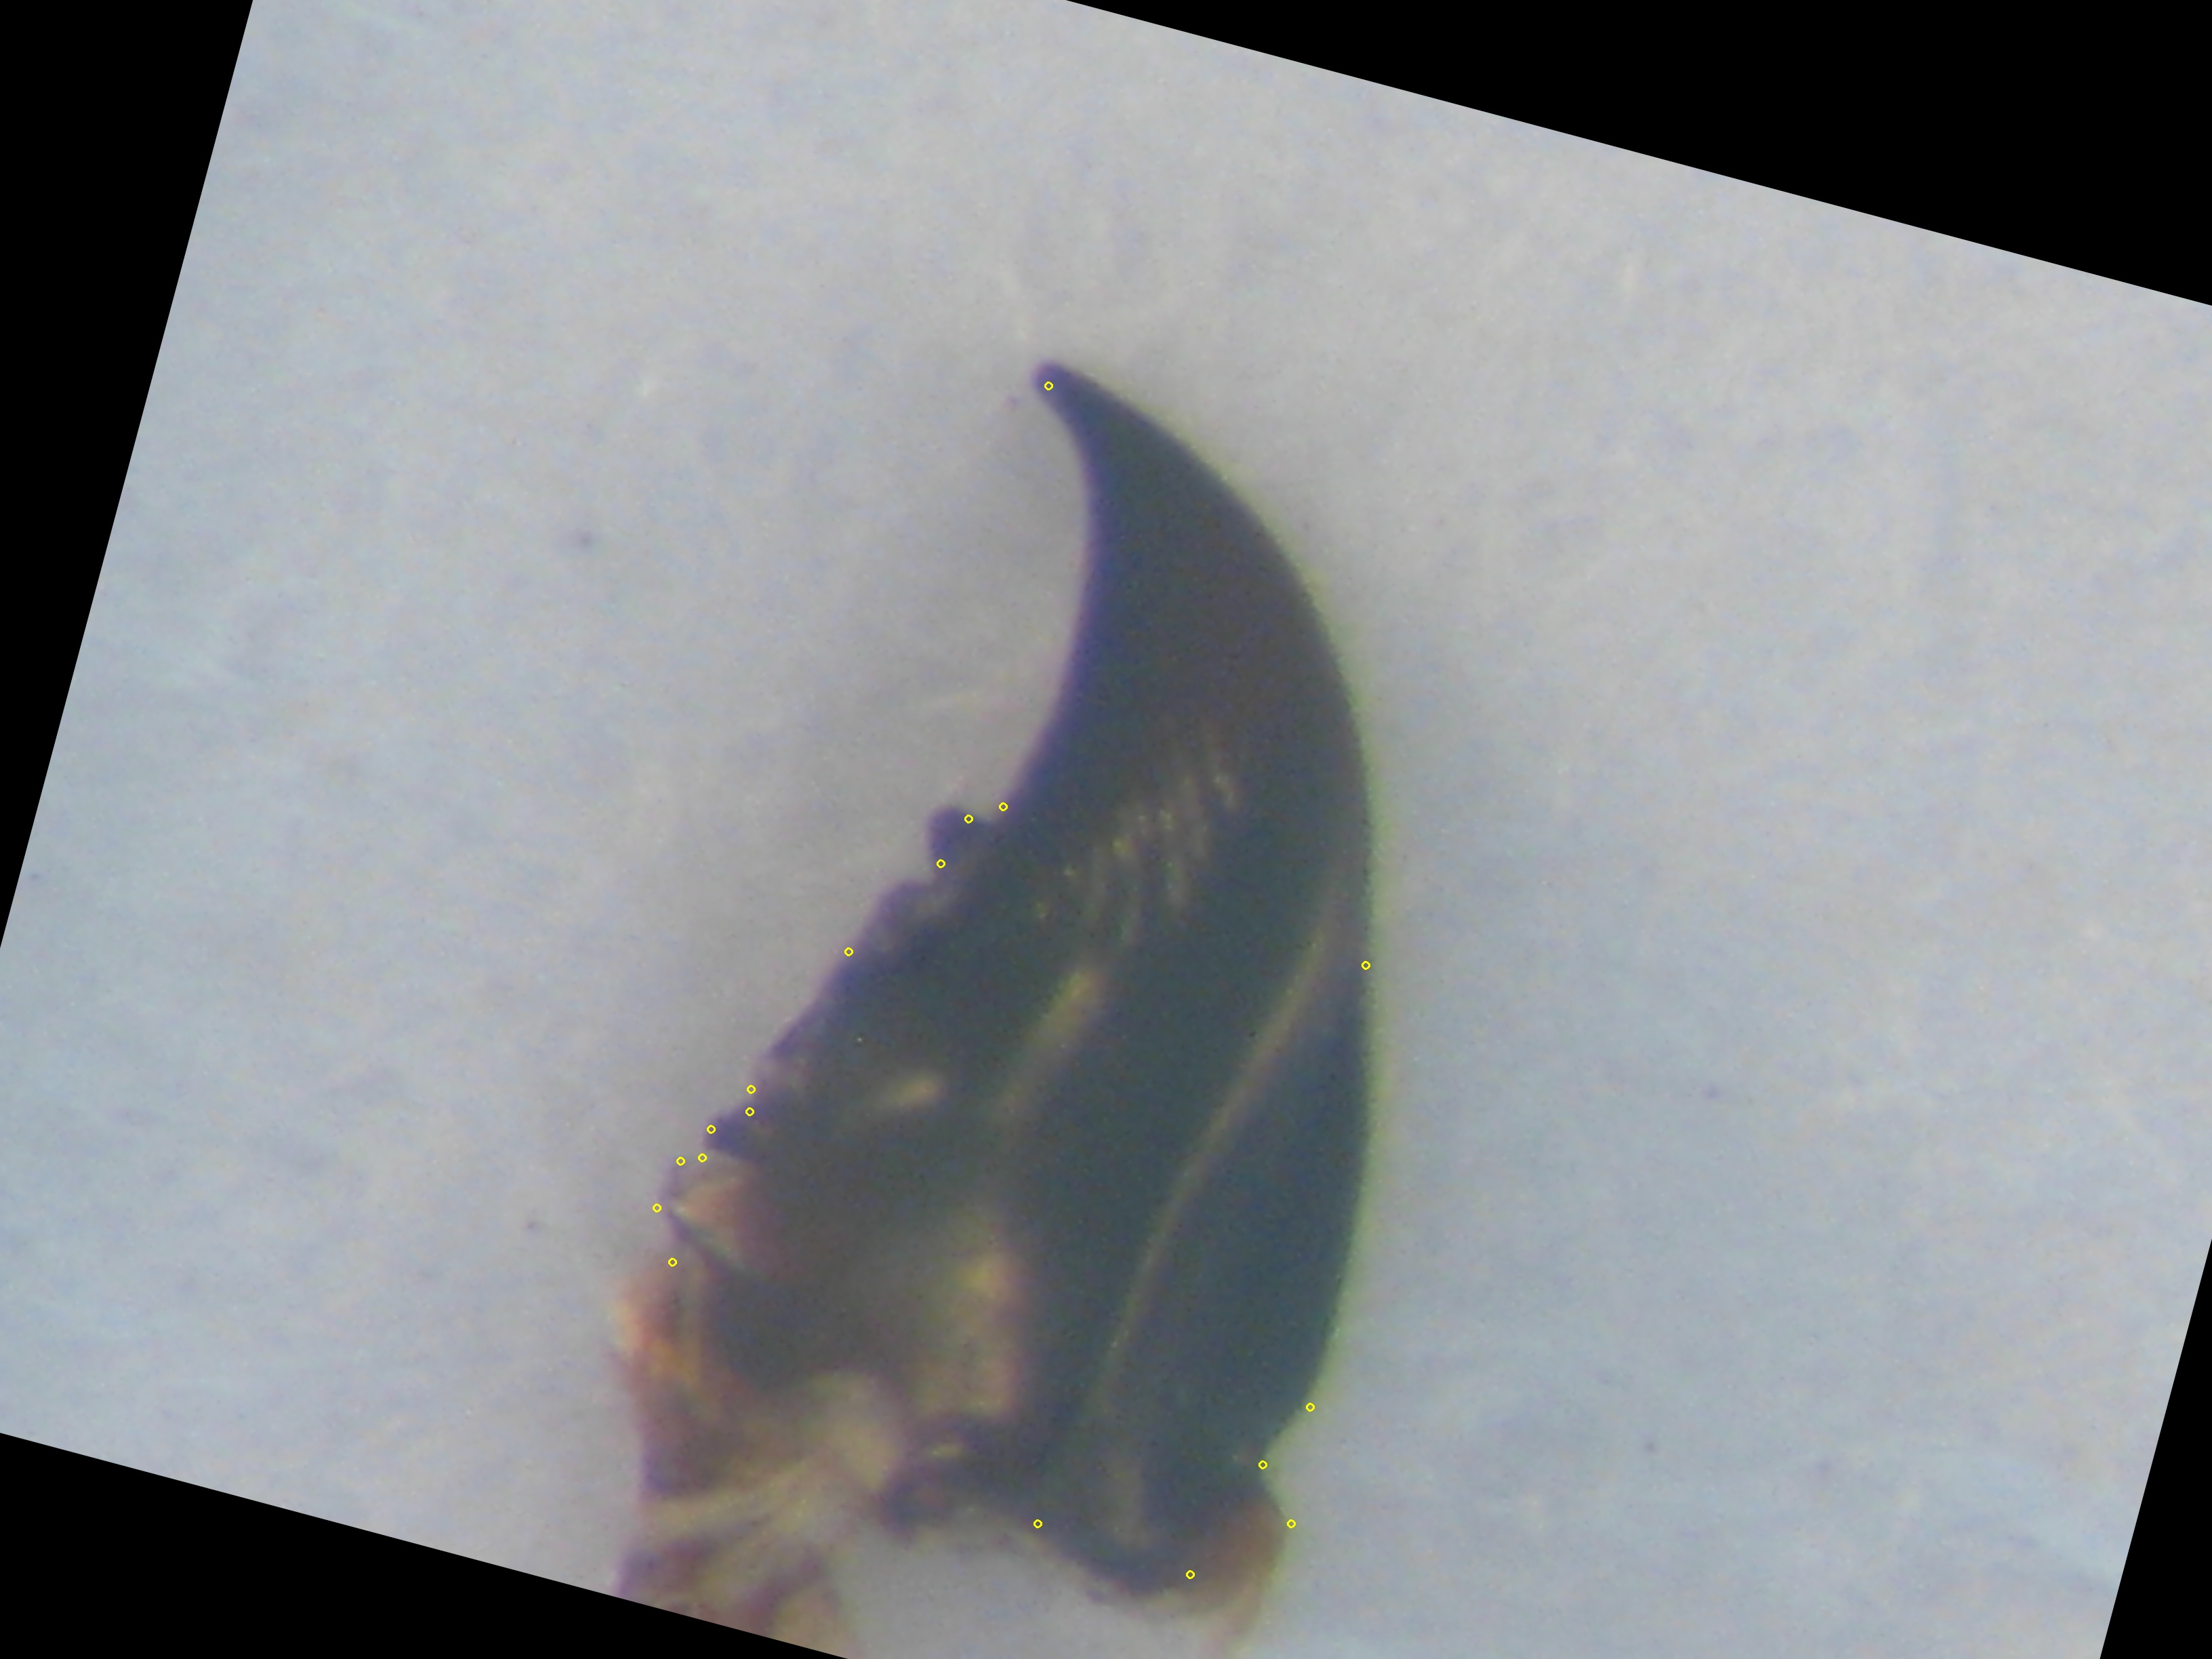
\includegraphics[width=0.45\textwidth]{./images/est32}}
\caption{Automatic identification the landmarks}
\label{fig:figure_31}

\end{figure}